\documentclass[conf]{new-aiaa}

\usepackage{amsmath,amssymb}
\usepackage{array}
\usepackage{float}
\usepackage{graphicx}
\usepackage{geometry}


\usepackage{float}
\usepackage{diagbox}
\usepackage[table,xcdraw]{xcolor}

\usepackage{siunitx}
\usepackage{longtable,tabularx}
\usepackage{caption}
\usepackage{subcaption}

\usepackage{minted}
\usemintedstyle{autumn}
\setminted{linenos,breaklines,tabsize=4,xleftmargin=1.5em}

\title{VE401 Term Project 2\\
Rules of metrological testing for net quantity of products in prepackage with fixed content}
\author{Group 21\\
Yihao Liu (515370910207)
\footnote{Authors' names are in alphabet order.}
}
\affil{University OF Michigan - Shanghai Jiao Tong University Joint Institute, Shanghai, China}

\begin{document}

\maketitle

\begin{abstract}
    
\end{abstract}

\vspace{11cm}
\noindent Keywords: 

\newpage

\tableofcontents
\newpage


\section{Nomenclature}

{\renewcommand\arraystretch{1.0}
\noindent\begin{longtable*}{@{}l @{\quad=\quad} l@{}}
$N$ & total number of inspection lot
\end{longtable*}}

\newpage

\section{Problem Statement}

\subsection{Introduction}

Fatal force and fatal shooting by police are topics that attract headlines and trigger heated debate around the world. When we are discussing these topics, it’s important to have a clear image of what ``fatal police shooting'' is. Then we will discuss the pattern of police shootings regarding to the probability. 

According to the statistics from the Washington Post [3] 962 people have been shot and killed by police in the US in 2016, and 994 people were fatally shot by police in 2015. The Washington Post is compiling such a database of every fatal shooting in the United States by a police officer in the line of duty since Jan. 1, 2015. This database is based on news reports, public records, social media and other sources.

For the term ``fatal police shooting,'' the Post characterizes it as those shootings in which a police officer, in the line of duty, shoots and kills a civilian — the circumstances that most closely parallel the 2014 killing of Michael Brown in Ferguson, Mo., which began the protest movement culminating in Black Lives Matter and attracted attention to police accountability nationwide [4]. What is worth attention is that the Post is not tracking deaths of people ``in police custody, fatal shootings by off-duty officers or non-shooting deaths.''

\begin{figure}[H]
	\centering
	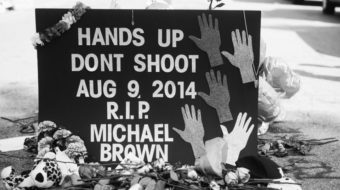
\includegraphics[width=0.7\linewidth]{intro.png}  
	\caption{Silent protest for police shooting of Michael Brown.}  
\end{figure}

Of course every single murder is a tragedy for those whom it affects, but for the bettering of the police service and the benefit of broader society we may wish to consider whether these ``shocking'' numbers lead to some patterns. In the following content, we carry out a statistical analysis on the mass shootings in the US from 2015 - 2018, exploring the distribution pattern, the dependence on weekday and month, then anticipating the number of police shootings in 2019.

\subsection{Overview}

First, we use \emph{Mathematica} to visualize the fatal police shooting from the data provided by \emph{WashingtonPost}\cite{} between January 1$^{\rm st}$,2015 and December 31$^{\rm st}$, 2018. The plot was shown in Figure \ref{fig:q2}.

\begin{figure}[H]
	\centering
	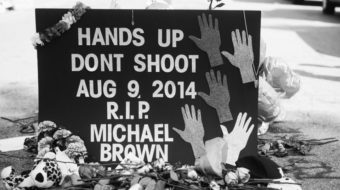
\includegraphics[width=0.9\linewidth]{intro.png}
	\caption{Number of fatal police shoots each day between January 1$^{\rm st}$,2015 and December 31$^{\rm st}$, 2018.}
	\label{fig:q2}
\end{figure}

Note that 2016 is a leap year, which means that it has one more day (February 29$^{\rm th}$) than the other three years, so the distance between 2016 and 2017 on the x-axis is slightly different from the distance between other years.

\subsection{Background}

In this project, we 

\newpage

\section{Description of work}

\subsection{Distribution of fatal police shooting each year}

In the work of Spiegelhalter and Barnett\cite{}, the London homicides follow a Poisson distribution with parameter $k = 0.44$. We think the distribution of fatal police shooting in the USA may be similar to that of London homicides, so we also assume that the police shootings follow a Poisson distribution with an unknown parameter $k$ and perform a goodness-of-fit test for a discrete distribution.



\subsection{q6}

Suppose that the number of fatal police shoot between January and March 2019 follows a Poisson distribution with unknown parameter $k$. We want
to determine if there is evidence that this claim is false.

According to the data obtained from xxx, there are 90 days in this three months, so that the random sample size is $N=90$.

\begin{tabular}{cc}
Number & Frequency \\\hline
0 & 8 \\
1 & 16 \\
2 & 22 \\
3 & 18 \\
4 & 11 \\
5 & 7 \\
6 & 5 \\
7 & 2 \\
8 & 0 \\
9 & 1 
\end{tabular}

(according to some proofs in q2 copied from example 2.2.7)

We know that a maximum-likelihood estimator for $k$ is the sample mean,
$$\hat{k}=\overline{X}=\frac{1}{90}
(0\cdot8+1\cdot16+2\cdot22+3\cdot18+4\cdot11
+5\cdot7+6\cdot5+7\cdot2+9\cdot1)=\frac{41}{15}.$$

In order to apply the multinomial distribution, we first calculate
\begin{align*}
P[X=0]&=\frac{e^{-\hat{k}}\hat{k}^0}{0!}=0.0650023\\
P[X=1]&=\frac{e^{-\hat{k}}\hat{k}^1}{1!}=0.177673\\
P[X=2]&=\frac{e^{-\hat{k}}\hat{k}^2}{2!}=0.24282\\
P[X=3]&=\frac{e^{-\hat{k}}\hat{k}^3}{3!}=0.221236\\
P[X=4]&=\frac{e^{-\hat{k}}\hat{k}^4}{4!}=0.151178\\
P[X=5]&=\frac{e^{-\hat{k}}\hat{k}^5}{5!}=0.0826438\\
P[X=6]&=\frac{e^{-\hat{k}}\hat{k}^6}{6!}=0.0376488\\
P[X\geqslant7]&=1-\sum_{i=0}^6P[X=i]=0.0217996
\end{align*}

expected frequencies:
5.8502, 15.9906, 21.8538, 19.9112, 13.606, 7.43794, 3.38839, 1.96196

Last two added and get 5.35036.

$$X^2=\sum_{i=1}^N\frac{(O_i-E_i)^2}{E_i}=2.81152$$
$$N-1-m=7-1-1=5$$
$$\chi^2_{0.72,5}=2.81$$

So the P-value of the test is 0.72, too large, unable to reject Poisson distribution

$$\hat{k}_{2019}=\frac{41}{15}$$

\newpage

\section{Test Results}


\begin{thebibliography}{9}
\bibitem{horst}Horst Hohberger, \emph{VE401,Probabilistic Methods in Eng. Slides}, University OF Michigan - Shanghai Jiao Tong University Joint Institute, Shanghai, China

\end{thebibliography}

\end{document}
